\documentclass[10pt]{article}
\usepackage[utf8]{inputenc}
\usepackage[english]{babel} % Language to be used
\usepackage[T1]{fontenc}
\usepackage{amsmath}
\usepackage{cite}  % Package to cite multiple references at once
\usepackage{url}
\usepackage{hyperref}
\usepackage[usenames,dvipsnames]{xcolor}
\usepackage{listings}
\usepackage{graphicx}
\usepackage{enumitem} 

\urlstyle{same} 

\lstset{
  basicstyle=\ttfamily,
  language=python,
  tabsize=4,
  frame=single,
  showstringspaces=false,
  showspaces=false,
  showtabs=false,
  captionpos=b,
  breaklines=true,
  breakatwhitespace=false,           % sets if automatic breaks should only happen at whitespace
  keywordstyle=\color{RoyalBlue},    % keyword style
  commentstyle=\color{ForestGreen},  % comment style
  stringstyle=\color{BrickRed}
}

% Parameters to the margins
\setlength{\topmargin}{-0.50in}
\setlength{\oddsidemargin}{-0.25in}
\setlength{\evensidemargin}{-0.25in}
\setlength{\textwidth}{7.0in}
\setlength{\textheight}{9.00in}

\title{\centering{MATH-6010: Your Project}}

\author{ \textbf{Name} \\
         your Unid}

\begin{document}
\date{\today}
\maketitle
\thispagestyle{empty}
% ----------------------------------------------------------------
\pagestyle{plain}
\pagenumbering{arabic}
\setcounter{page}{1}
\renewcommand \thesection{\Roman{section}}

%\include{intro}
\section{Data Retrieval}
Our data sets (\textbf{Medical Cost Personal Datasets}) were obtained from the \texttt{Kaggle} website\cite{kaggle:2022a}.

The data set has six independent variables:
\begin{enumerate}
\item \texttt{age} 
\item \texttt{sex} 
\item \texttt{bmi} 
\item \texttt{children} 
\item \texttt{smoker}
\item \texttt{region}	
\end{enumerate}
and one dependent variable: \texttt{charge}.

In Fig.\,\ref{fig:chargesfuncofbmi} the charges (\$) as function of bmi are displayed.
\begin{figure}[h]
   \centering
	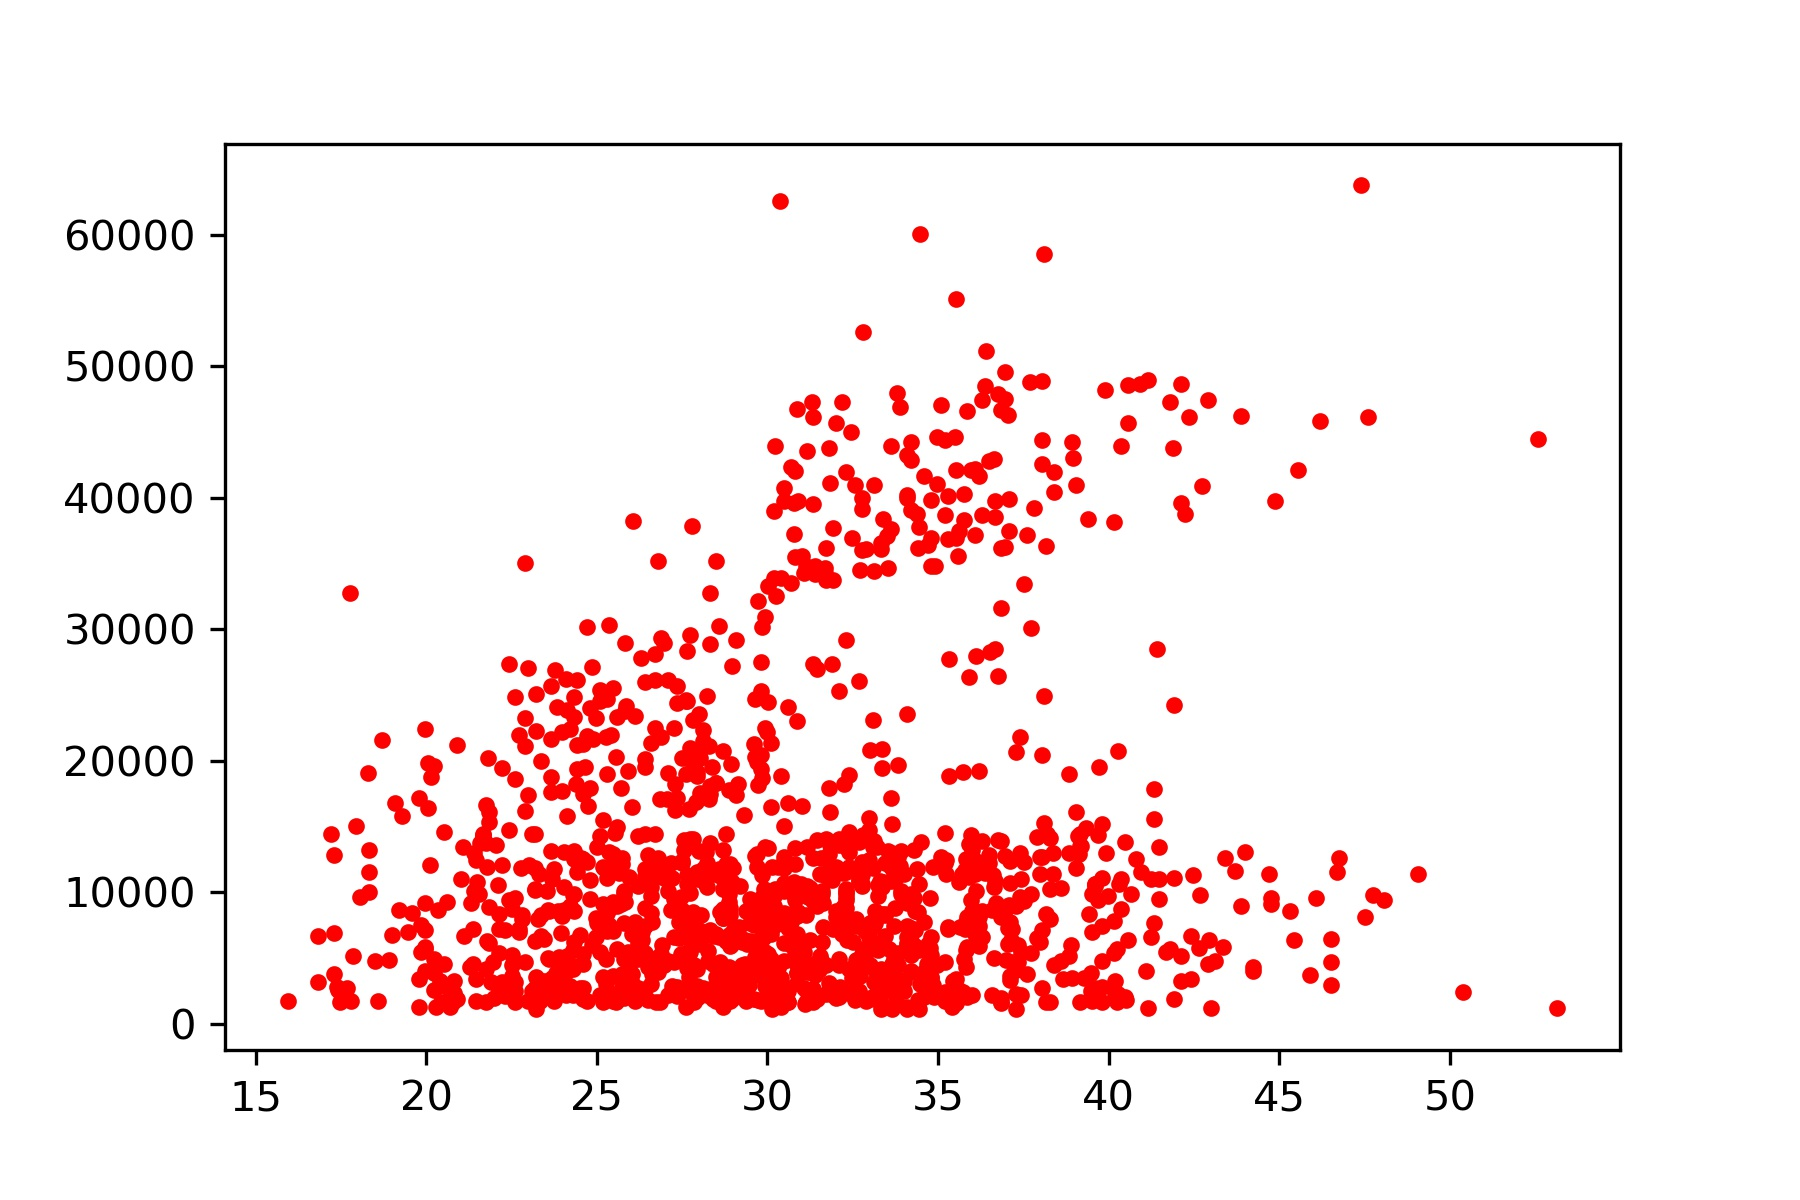
\includegraphics{../img/imgpy1.jpeg}
	\caption{Charges (\$) as function of bmi.}
  \label{fig:chargesfuncofbmi}
\end{figure}

In Fig.\,\ref{fig:countsofage} the age histogram is displayed.
\begin{figure}[h]
   \centering
        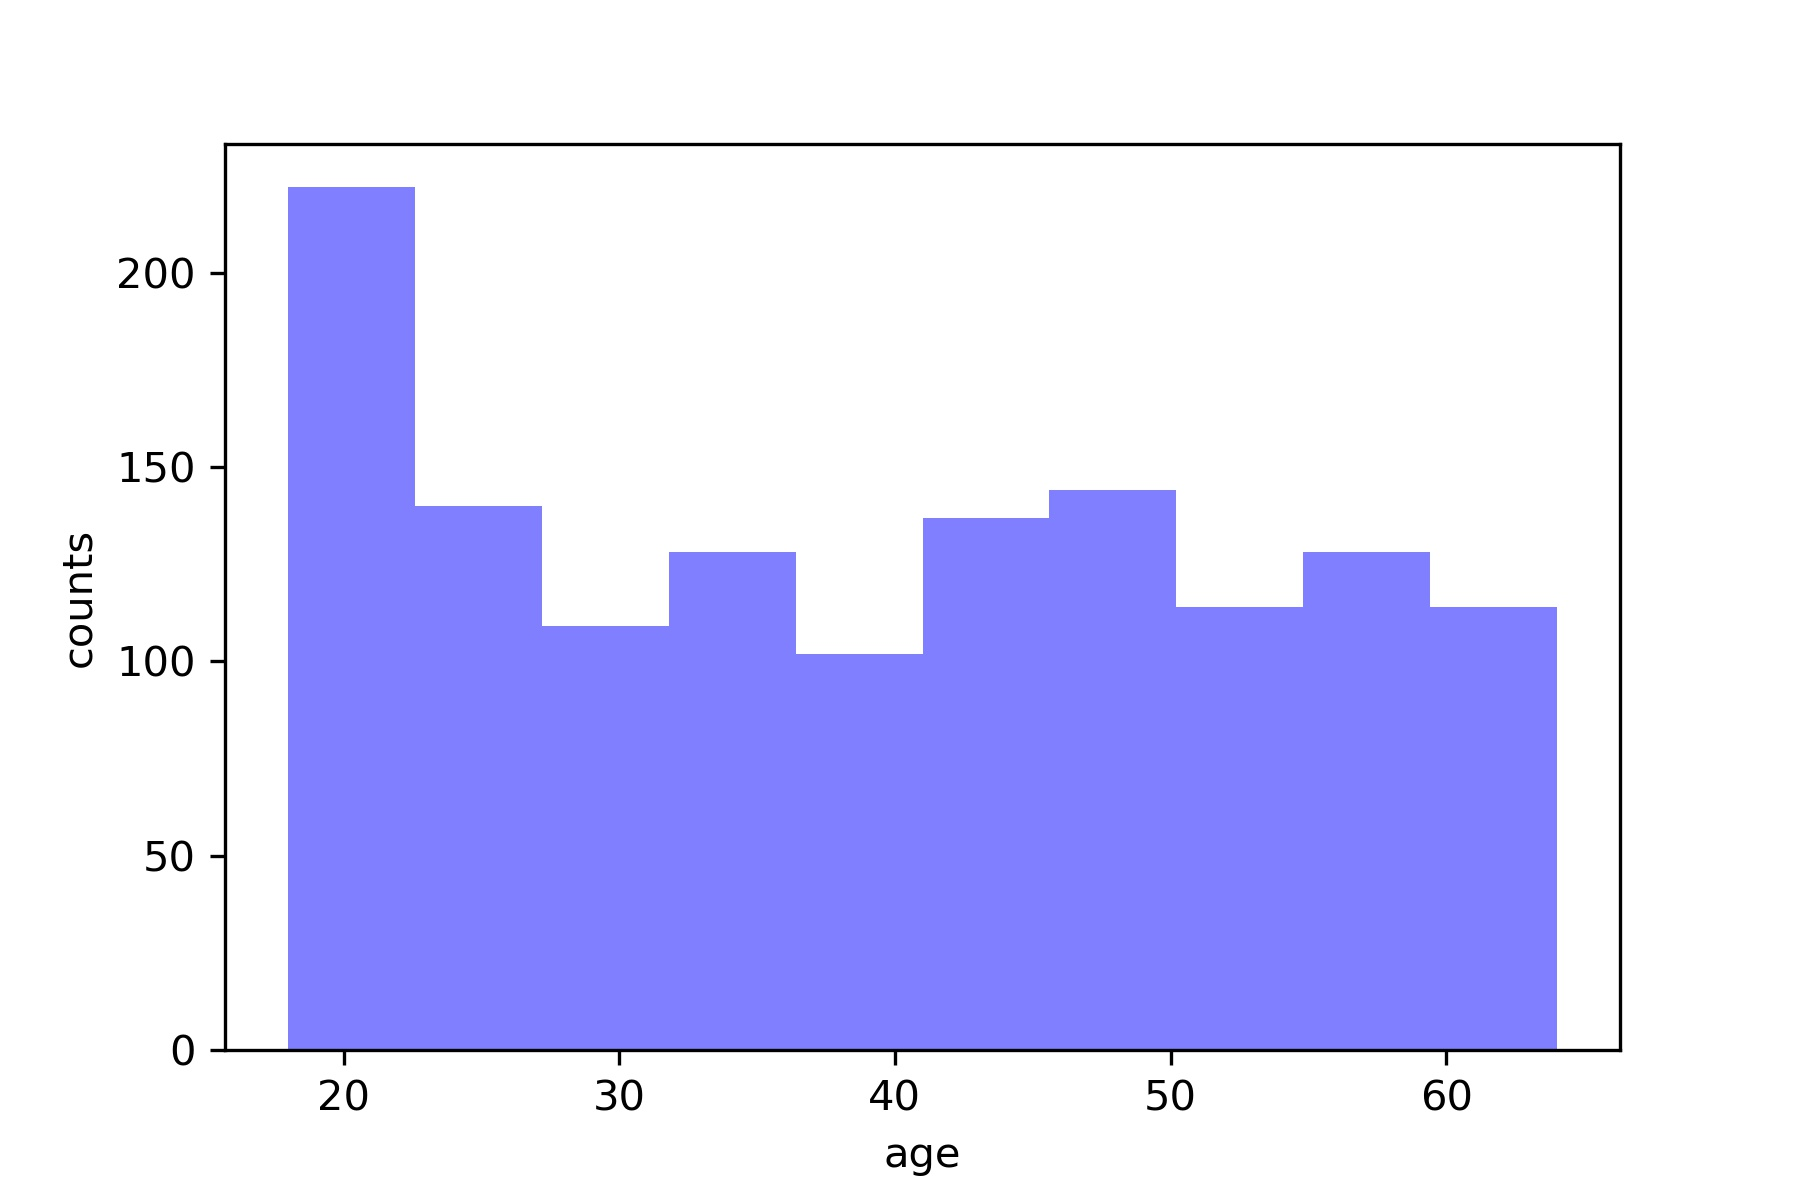
\includegraphics{../img/imgpy2.jpeg}
        \caption{Age histogram.}
  \label{fig:countsofage}
\end{figure}


\section{Statistical Analysis}

\subsection{Model}
In what follows we will use the following linear model:
\begin{eqnarray}
       Y_i & = & \beta_0 \, + \, x_{i,1}\,\beta_1 \,+\,
                 x_{i,2}\,\beta_2 \, + \,x_{i,3}\,\beta_3 \,+\,
                 x_{i,4}\,\beta_4 \, + \, \epsilon_i \nonumber \\
	   & = & \displaystyle \sum_{k=0}^4 x_{i,k}\,\beta_k \, + \, \epsilon_i \label{Eqn:Model1}		 
\end{eqnarray}
where $x_{i,0}:=1$.

Eq.\,(\ref{Eqn:Model1}) can also be rewritten in matrix form\footnote{In what follows we will display vectors in bold.}:
\begin{eqnarray}
        \boldsymbol{Y} & = & \boldsymbol{X} \, \boldsymbol{\beta} \, + \, \boldsymbol{\mathcal{E}} \label{Eqn:Model2}
\end{eqnarray}


The test of the null hypothesis can be achieved by calculating the value for the following F-statistic\,\cite{seber2012linear}:
\begin{eqnarray}
        f_{1,n-p} & = & \frac{ \boldsymbol{(A\widehat{\beta}\,-\,c)^T}  \,
                        \boldsymbol{\Bigg[ A(X^TX)^{-1}A^T \Bigg]^{-1} } \,
                          \boldsymbol{(A\widehat{\beta}\,-\,c)}
                         }{S^2} \label{Eq:Fstatistic}
\end{eqnarray}
where the expression $\boldsymbol{(A\widehat{\beta}\,-\,c)}$
imposes a constraint on $\boldsymbol{\widehat{\beta}}$.

%\include{aux}
% ---------------------------------
\newpage
\bibliographystyle{amsplain}
\bibliography{template}
%\newpage
%\include{appendix}

\end{document}
